\section{Diagrama de bloques (hardware)}
\label{sec:diag_bloq}
A continuación se muestra el diagrama de bloques del sistema utilizado. El microcontrolador puede recibir o establecer el tipo de desplazamiento que se desea aplicar sobre el parlante. Dicho modo de desplazamiento puede ser recibido mediante la interfaz USB/Serie que vincula al microcontrolador con la PC, como también ser seleccionado a través de un teclado (pulsadores) conectado al microcontrolador, donde el usuario elegirá el tipo de desplazamiento a realizar mediante las opciones vistas en el display, y será el microcontrolador el encargado de efectuarlas, a diferencia de la otra forma, donde solo actuará como intermediario.

\begin{figure}[H]
  \centering
  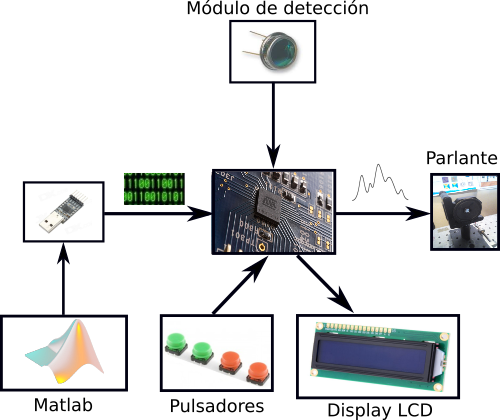
\includegraphics[width=1.0\textwidth]{images/diagrama_de_bloques.png}
  \caption{Diagrama de bloques que muestra cómo interactúan los diferentes dispositivos que conforman el proyecto.}
  \label{fig:Diagrama de bloques}
\end{figure}